\PassOptionsToPackage{unicode}{hyperref}
\PassOptionsToPackage{hyphens}{url}
%
\documentclass[12pt, a4paper]{article}
% NOTE: the course page requires 3cm margins (the original template had 1in)
\usepackage[a4paper,margin=3cm]{geometry}
\setlength\parindent{0pt}
\usepackage{mathptmx}
\usepackage{amsmath,amssymb}
\usepackage[T1]{fontenc}
\usepackage[utf8]{inputenc}
\usepackage{textcomp}
\usepackage{booktabs}   % nicer tables
\usepackage{graphicx}   % figures

\author{Name1 Surname1, Degree Programme, ID number (matricola)
\\Name2 Surname2, Degree Programme, ID number (matricola)
\\Name3 Surname3, Degree Programme, ID number (matricola)
\\Name4 Surname4, Degree Programme, ID number (matricola)
\\Name5 Surname5, Degree Programme, ID number (matricola)}
\date{}
\title{Formal Departments and Informal Communication:\\
A Network Analysis of E-mail in a European Research Institution}

\begin{document}
\maketitle

\section{Introduction}
\label{introduction}

This project uses social network analysis to study communication inside an
organisation. In particular, we analyse the e-mails exchanged among the members
of a European research institution.

An organisation can be described in two ways. The first is its official
structure: every person belongs to a department, and departments are the units
where work is organised. The second is how people really work together: whom
they talk to and exchange information with. These two do not always match,
because people often need to work with colleagues outside their own department.
E-mail data is a good way to observe the second structure: it is recorded
automatically, it covers the whole organisation, and, unlike a survey, it does
not depend on what people remember \cite{borgatti2018}.

The dataset we use was published together with studies on how networks grow
over time \cite{leskovec2007} and on algorithms that find groups in a network
\cite{yin2017}. The second study uses the department of each person to check
whether an algorithm finds the right groups. We use the same information for a
different goal: to compare the official departments with the way people
actually communicate.

\section{Problem and Motivation}
\label{problem-and-motivation}

The problem we study is whether the division of a research institution into
departments affects whom its members e-mail, and how much. This question is
interesting for two reasons. In theory, it checks whether the official borders
between departments are also borders for communication. In practice, it shows
where information moves easily and where it may get stuck: a department whose
members write only to each other can become isolated, while the few people who
connect different departments become very important, because information
between departments depends on them.

We split the problem into three research questions:
\begin{itemize}
  \item \textbf{RQ1:} What is the overall structure of the e-mail network, and
        do departments differ structurally?
  \item \textbf{RQ2:} Who are the central actors, and who bridges departments?
  \item \textbf{RQ3:} Are departments real boundaries of communication?
\end{itemize}

RQ1 looks at the network as a whole: how connected it is, whether people answer
each other's e-mails, and how fast information can spread. RQ2 looks at single
people and finds who has the most important positions. RQ3 directly compares
the departments with the groups that appear from the e-mails.

The main contributions of the project are:
\begin{itemize}
  \item a description of the structure of the whole institution and of its four
        largest departments, where the main measures are compared with random
        networks of the same size;
  \item a list of the most central members and of the people who connect
        different departments;
  \item a statistical test of whether people in the same department e-mail each
        other more, and a comparison between the groups found from the e-mails
        and the official departments.
\end{itemize}

\section{Datasets}
\label{datasets}

% TODO (Person 2)
How did you gather the data? Did you digitise it? How? Is the material
publicly available? What tools did you use 1) to handle (store,
manipulate) the data and 2) to compute measures on the data?

\section{Validity and Reliability}
\label{validity-and-reliability-not-needed-for-the-project-proposal}

% TODO (Person 3)
How closely does the model of your dataset represent reality (validity)?
How does the way you treat the data affect the reproducibility of the study (reliability)?

\section{Measures and Results}
\label{measures}

% ------------------------------------------------------------------
\subsection{Network structure (RQ1)}
\label{sec:structure}
% ------------------------------------------------------------------

To answer RQ1 we describe the structure of the whole network and compare it
with the four largest departments (IDs 4, 14, 1 and 21). Each department is
analysed as the network of e-mails sent among its own members. All measures
were computed with NetworkX and are shown in Table~\ref{tab:structure}.
Clustering and distance measures are usually computed on undirected networks,
so for these we made the networks undirected with the OR rule (two people are
linked if at least one of them e-mailed the other). We computed distances only
on the largest connected component (LCC), because there is no distance between
people who are not connected.

\textbf{Density and reciprocity.} We first look at how many connections exist
and whether links go in both directions. Density, the share of all possible
sender--receiver pairs that really exist, is low in the whole network (0.025):
on average a member writes to about 25 of the other 1{,}004 members. In the
departments density is four to seven times higher (0.099--0.180). A group of
the same size chosen at random from the institution would have about the same
density as the whole network, so this difference is not an effect of size:
members write much more to colleagues of their own department than to other
members, a result tested in Section~\ref{sec:departments}. Reciprocity, the
share of links that also exist in the opposite direction, is high everywhere
(0.68--0.82). In a random network it would be equal to the density (0.025 for
the whole network), so it is about 28 times higher than chance. Most e-mail
links therefore go both ways: when a person writes to a colleague, the
colleague usually also writes to them. Department~21 has the highest
reciprocity.

\textbf{Connectivity.} If we ignore the direction of e-mails, 98.1\% of the
members are in one connected component, so almost everyone is linked to
everyone else through a chain of colleagues. If we follow the direction of
e-mails, the largest strongly connected component includes 79.9\% of the
members. Of the other 20.1\%, 19 members (1.9\%) send and receive no e-mail at
all, while the rest are linked to this group but cannot both reach it and be
reached from it. Inside departments the network is less connected. In
departments~1 and~21 only about half of the members (58.5\% and 52.5\%) can
reach each other by following e-mails, and 13.8\% and 24.6\% of the members
are outside the department LCC. These members are not all in the same
situation: some e-mail only people of other departments, some send no e-mail at
all, and a few form a small separate group (Section~\ref{sec:departments}).

\textbf{Small-world structure.} Next, we check whether the network has close
groups of colleagues and, at the same time, short paths between people. This is
called the small-world property \cite{watts1998}. We measure how close the
groups are with the average clustering coefficient, the probability that two
contacts of a person are also linked. We measure how far people are with the
average shortest path length, the average number of steps between two people
\cite{newman2018}. These numbers only make sense if we compare them with random
networks of the same size, so for each network we computed the average over
ten random Erdős–Rényi networks $G(n,m)$ with the same number of nodes and
edges. In the whole network the clustering is 0.407, against 0.033 in the
random networks (about twelve times higher), while the average path is only a
little longer (2.59 against 2.30) and the diameter is 7. Ignoring the direction
of e-mails, two connected members are therefore on average less than three
steps apart, even though people form close groups. The coefficient
$\sigma = (C/C_{rand})/(L/L_{rand})$ is 10.8; values above 1 indicate a
small-world network. Transitivity, the share of closed triangles in the whole
undirected network, is lower (0.267) than the average clustering, because the
contacts of very active members are less often linked to each other than the
contacts of other members.

Because $\sigma$ becomes larger when the network is bigger, we compared the
departments with two other measures. First, the ratio $C/C_{rand}$ shows how
much more clustered a department is than chance: department~4 is the most
clustered (3.2 times the random value), followed by departments~1 (2.8), 14
(2.1) and 21 (1.9). The raw clustering gives the opposite order, because small
and dense departments have high clustering even at random. Second, we used the
coefficient $\omega$ as implemented in NetworkX, which compares the network
with 10 random networks that keep the degree of every node and with 10
lattice-like networks. It is close to 0 for small-world networks, negative for
networks similar to a regular grid (lattice) and positive for networks similar
to random ones. All four departments have $\omega$ close to 0 (from $-0.11$ to
$+0.06$), so they are also small-world networks. Department~1 has the lowest
value ($\omega=-0.11$), so it is the most similar to a lattice, but the
difference is small.

\textbf{Degree distribution.} Finally, we check whether contacts are spread
evenly or concentrated in a few people. Figure~\ref{fig:degree} shows the
in-degree (from how many colleagues a person receives e-mails) and the
out-degree (to how many colleagues a person writes) on log-log axes. In the
whole network both distributions have a long tail: most members have a small or
moderate number of contacts, while a few have more than 100 (up to about 210
for in-degree and more than 300 for out-degree). These members are good
candidates for the central roles studied in Section~\ref{sec:centrality}. We
did not test whether the network is scale-free by fitting a power law, because
with about 1{,}000 nodes there are too few points in the tail for a reliable
result \cite{newman2018}; we only say that the distribution has a long tail.
The department networks are too small to show a clear shape.

\begin{table}[ht]
\centering
\small
\begin{tabular}{lrrrrr}
\toprule
 & Whole & Dept 4 & Dept 14 & Dept 1 & Dept 21 \\
\midrule
Nodes                         & 1005  & 109   & 92    & 65    & 61    \\
Edges (directed)              & 24929 & 1167  & 1506  & 502   & 601   \\
Density                       & 0.025 & 0.099 & 0.180 & 0.121 & 0.164 \\
Reciprocity                   & 0.711 & 0.723 & 0.708 & 0.681 & 0.819 \\
Mean in/out degree            & 24.81 & 10.71 & 16.37 & 7.72  & 9.85  \\
LCC share of nodes            & 0.981 & 0.927 & 0.967 & 0.862 & 0.754 \\
Largest SCC share             & 0.799 & 0.789 & 0.859 & 0.585 & 0.525 \\
Transitivity                  & 0.267 & 0.424 & 0.457 & 0.545 & 0.665 \\
Avg.\ clustering $C$          & 0.407 & 0.471 & 0.520 & 0.587 & 0.660 \\
Random avg.\ clustering $C_{rand}$ & 0.033 & 0.147 & 0.249 & 0.213 & 0.344 \\
Avg.\ shortest path $L$       & 2.587 & 2.165 & 1.830 & 2.450 & 1.788 \\
Random avg.\ shortest path $L_{rand}$ & 2.296 & 1.948 & 1.754 & 1.852 & 1.660 \\
Diameter                      & 7     & 5     & 4     & 5     & 4     \\
$\sigma$                      & 10.84 & 2.88  & 2.00  & 2.08  & 1.78  \\
$\omega$                      & --    & $0.063$ & $0.063$ & $-0.106$ & $-0.014$ \\
\bottomrule
\end{tabular}
\caption{Structural measures of the whole network and of the four largest
departments. Density, reciprocity and SCC share use the directed network;
transitivity uses the whole undirected (OR) network; average clustering, path
lengths, diameter, $\sigma$ and $\omega$ use the undirected largest connected
component. Random baselines average ten $G(n,m)$ networks of the same size.
$\omega$ was not computed for the whole network because of its computing time.}
\label{tab:structure}
\end{table}

\begin{figure}[ht]
\centering
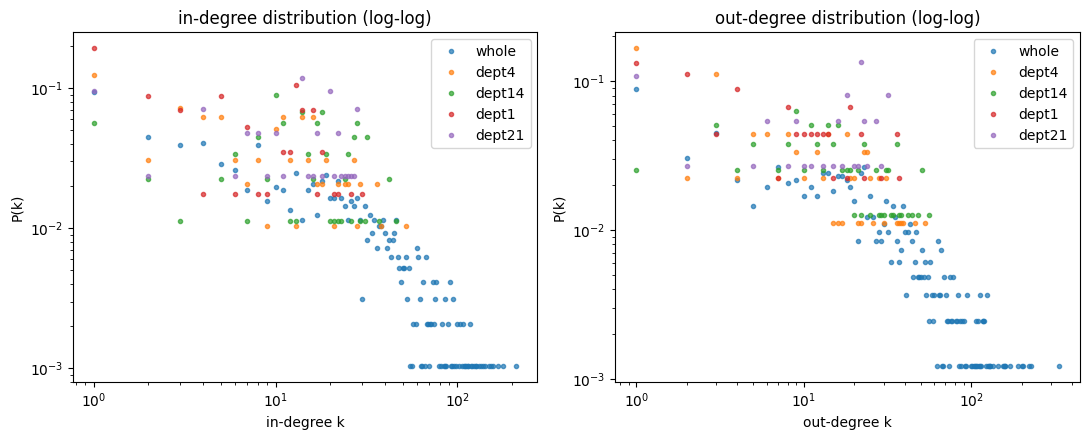
\includegraphics[width=\textwidth]{degree_distribution.png}
\caption{In-degree (left) and out-degree (right) distributions on log-log
axes for the whole network (blue) and the four largest departments (other
colours; ``dept4'' = Department~4). Members with degree 0 are not shown. The
whole network has a long tail: a few members have more than 100 contacts.}
\label{fig:degree}
\end{figure}

% ------------------------------------------------------------------
\subsection{Central actors and bridges (RQ2)}
\label{sec:centrality}
% TODO (Person 2)

% ------------------------------------------------------------------
\subsection{Departments as communication boundaries (RQ3)}
\label{sec:departments}
% TODO (Person 3)


\section{Conclusion}
\label{conclusion}

\subsection{RQ1: network structure}
The e-mail network of the institution is a small-world network: members form
close groups, yet, ignoring the direction of e-mails, two connected members are
on average less than three steps apart, and most e-mail links go both ways.
This structure can support both teamwork inside groups and the fast spread of
information in the whole institution. The four largest departments share the
same basic pattern: they are small-world and highly reciprocal. They differ,
however, in how clustered they are compared with chance (department~4 the
most, department~21 the least) and in how connected they are: in
departments~1 and~21 only about half of the members can reach each other by
following e-mails. Department density is four to seven times the density of the
institution, and in department~21 one member in six (10 of 61) e-mails only
people of other departments. Departments therefore matter for communication,
but they do not contain all of it.

% TODO 6.2 (Person 2), 6.3 (Person 3)

\section{Critique}
\label{critique}

\subsection{RQ1: network structure}
This part of the study has three limits. First, the network only records
whether two people exchanged at least one e-mail over the whole period, so one
single message counts as much as daily contact, and a short path in the network
may not be possible in time order. A weighted network built from the version
of the dataset with timestamps would show how strong and when each connection
is. Second, the $G(n,m)$ random networks give every member a similar number of
contacts, while real degrees are very uneven; random networks that keep the
real degrees, as used for $\omega$, are a stricter baseline, but we could not
compute them for the whole network because of the computing time. Third, the
department networks are small (61--109 members) and keep only the e-mails
inside each department, so their results are less certain and say nothing
about contacts with other departments, which are studied in
Section~\ref{sec:departments}.

% TODO 7.2 (Person 2), 7.3 (Person 3)

\begin{thebibliography}{99}
\bibitem{borgatti2018} S.~P. Borgatti, M.~G. Everett, J.~C. Johnson.
  \emph{Analyzing Social Networks}. Sage, 2018.
\bibitem{leskovec2007} J.~Leskovec, J.~Kleinberg, C.~Faloutsos. Graph evolution:
  densification and shrinking diameters. \emph{ACM Transactions on Knowledge
  Discovery from Data}, 1(1), 2007.
\bibitem{newman2018} M.~Newman. \emph{Networks}. Oxford University Press, 2018.
\bibitem{watts1998} D.~J. Watts, S.~H. Strogatz. Collective dynamics of
  `small-world' networks. \emph{Nature}, 393:440--442, 1998.
\bibitem{yin2017} H.~Yin, A.~R. Benson, J.~Leskovec, D.~F. Gleich. Local
  higher-order graph clustering. In \emph{Proceedings of the 23rd ACM SIGKDD
  International Conference on Knowledge Discovery and Data Mining}, 2017.
\end{thebibliography}

\end{document}
